\section{Evaluation}
\label{section:evaluation}
\subsection{Experimental Setup}
\label{subsec:setup}

\paragraph{Base model.}
We use Code World Model (CWM), a state-of-the-art open-weight 32B code LLM for agentic software engineering, as our base model. Specifically, we utilize the \cwm-sft~\cite{cwmsft} checkpoint, which is obtained prior to its joint RL stage.
This allows us to build on a checkpoint that has not been influenced by RL and fairly evaluate different learning strategies.
We use the same LLM for bug generation and repair, where the shared policy weights are updated continuously during RL.

\paragraph{Evaluation setup.}
We conduct evaluation on \sbv~\cite{swebverified}, a subset of \swebench~\cite{swebench} with 500 human-verified real-world software issues, and \sbp{} (public split)~\cite{deng2025swebenchproaiagents},  which contains 731 publicly available software problems, aimed to capture realistic, complex, and enterprise-level tasks.
We perform one attempt for each problem without parallel test-time scaling or ranking.
We use temperature $= 1.0$ and $\textrm{top-p} = 0.95$ for evaluation.

\subsection{Baseline Comparison}
\begin{figure*}[htb!]
    \centering
    \begin{subfigure}{0.38\linewidth}
        \centering
        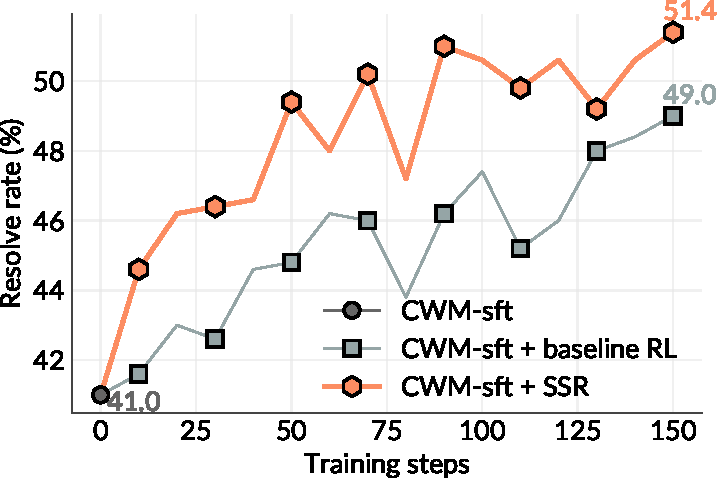
\includegraphics[width=\linewidth]{plots/ssr_vs_baseline_sbv.pdf}
        \caption{\sbv}
        \label{fig:baseline:sbv}
    \end{subfigure}%
    \quad%
    \begin{subfigure}{0.38\linewidth}
        \centering
        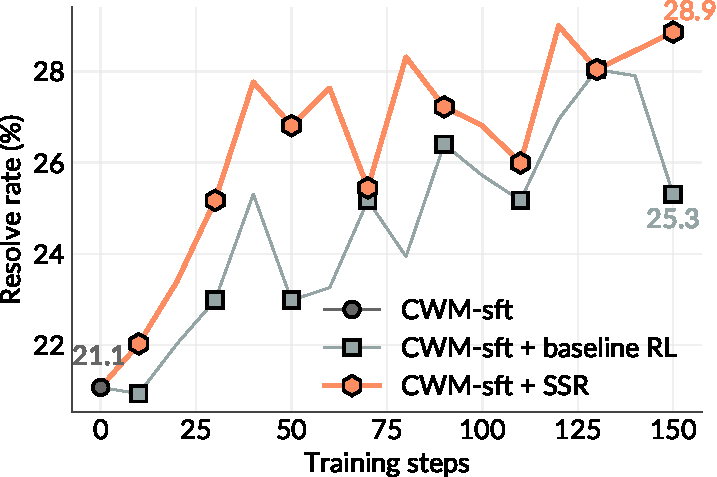
\includegraphics[width=\linewidth]{plots/ssr_vs_baseline_sbp.pdf}
        \caption{\sbp}
        \label{fig:baseline:sbp}
    \end{subfigure}
    \caption{Baseline comparison over the course of training.}
    \label{fig:baseline}
\end{figure*}
We compare the base model, baseline RL, and \tech on the \sbv and \sbp benchmarks.
Both baseline RL and \tech train on an identical set of environment images.
The fundamental difference lies in what information each approach can access.
Baseline RL, like standard agentic RL in \cwm~\cite{faircodegenteam2025cwmopenweightsllmresearch}, has access to natural language issue descriptions, pass-to-pass and fail-to-pass tests, and evaluation scripts, so the RL process simply checks whether solutions pass the given tests.
In contrast, \tech operates with only bare environment images, requiring the model to discover problems, formulate solutions, and validate them entirely through self-play without any provided descriptions or tests.

\Cref{fig:baseline} presents the results. We first observe that \tech achieves steady self-improvement throughout training, despite having no access to task-specific training data. This demonstrates that LLMs can self-improve their software engineering ability, such as issue-solving, purely through interaction with raw codebases. Furthermore, \tech consistently outperforms baseline RL on both benchmarks across the entire training trajectory, indicating that self-generated tasks provide richer and more effective learning signals than human-engineered data.


\subsection{Ablation of Self-Play Components}
\label{sec:ablate:components}

\begin{figure*}[htb!]
    \centering
    \begin{subfigure}{0.32\linewidth}
        \centering
        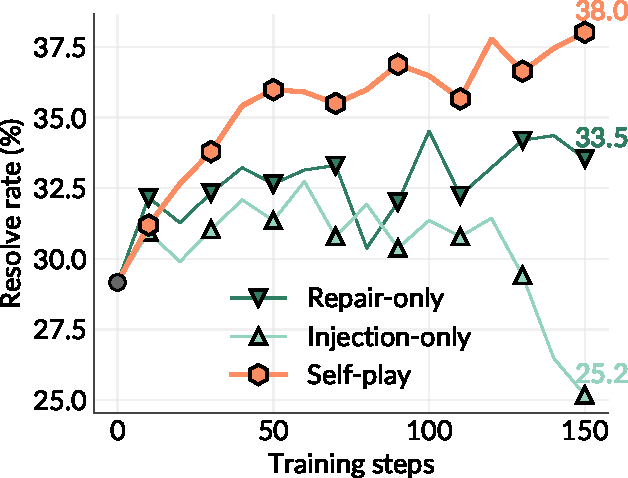
\includegraphics[width=\linewidth]{plots/ssr_role_ablation_both.pdf}
        \caption{Self-play components}
        \label{fig:role_ablate}
    \end{subfigure}%
    \hfill%
    \begin{subfigure}{0.32\linewidth}
        \centering
        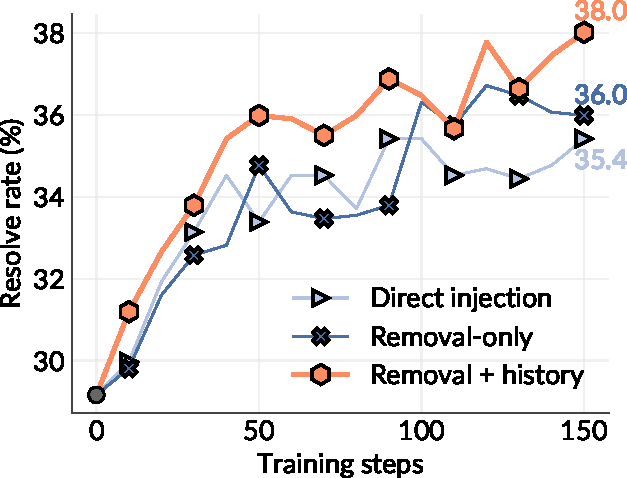
\includegraphics[width=\linewidth]{plots/ssr_prompt_ablation_both.pdf}
        \caption{Bug-injection methods}
        \label{fig:prompt_ablate}
    \end{subfigure}%
    \hfill%
    \begin{subfigure}{0.32\linewidth}
        \centering
        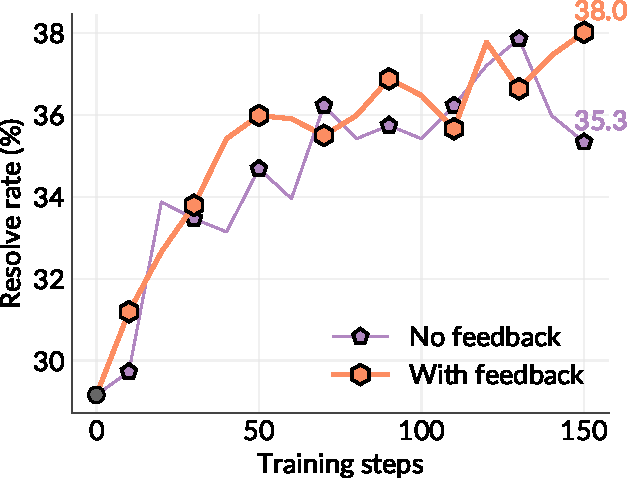
\includegraphics[width=\linewidth]{plots/ssr_reward_ablation_both.pdf}
        \caption{Solver feedback in bug-injection}
        \label{fig:reward_ablate}
    \end{subfigure}
    \caption{Ablation studies. The resolve rate is averaged over 1231 tasks from 500 \sbv and 731 \sbp tasks.}
    \label{fig:all_ablations}
\end{figure*}


To isolate the contribution of self-play, we compare the \tech with an injection-only and a repair-only variant, both trained using standard RL.
In the injection-only setting, the agent is only trained for bug generation, still using the \tech reward but with no training signal from repair trajectories;
for repair-only, the agent is exclusively trained to solve bugs, where the bug data comes from the valid, solvable, and deduplicated bugs from prior self-play runs.

\Cref{fig:role_ablate} shows that self-play is the best.
Injection-only training degrades the performance since it does not learn from any bug-solving attempts.
Repair-only training is also inferior because it lacks the evolving task distribution produced by self-play. In contrast, self-play requires the agent not only to repair bugs but also to propose challenging ones, which itself embodies substantial learning: identifying passing tests, breaking functionality in meaningful ways, and weakening tests to hide the bug. These activities continually expand the training signal and expose the model to new failure modes.
These results indicate that an evolving and online process of bug generation and bug solving is essential for sustained improvement.


\subsection{Ablation of Bug Injection Methods}


We also study how different bug-injection strategies affect downstream performance. \Cref{fig:prompt_ablate} compares three variants (full prompts in \cref{sec:apd:prompt_bug_injection}):
\begin{itemize}
\item \textbf{Direct-injection}: naive prompting to introduce bugs without detailed guidance.
\item \textbf{Removal-only}: instructing the agent to remove substantial code hunks or files while ensuring the project remains runnable.
\item \textbf{Removal + history}: randomly sampling between two prompts, one using the removal-only strategy and the other using a history-aware strategy that reverts selected historical changes from git logs.
\end{itemize}

From the figure, \tech proves effective across all injection strategies, demonstrating its generalizability. However, the effectiveness of different methods varies in subtle but meaningful ways.
First, direct-injection leads to the worst result because it tends to produce trivial bugs with superficial one-line modifications (e.g., \texttt{var = 0} $\to$ \texttt{var = 1}) that offer little training signal.
By contrast, the removal-only strategy generates stronger bugs, forcing the solver to reconstruct missing functionality and thereby deepening its understanding of repository structure.
Finally, ``removal + history'' achieves the best overall performance by leveraging more historical changes that incorporate more realistic and diverse bug patterns.
These findings highlight the importance of carefully designing bug-injection mechanisms for a more challenging and instructive curriculum.


\subsection{Reward Ablation}
As discussed in \cref{sec:bug_injection}, the bug-injection reward incorporates feedback from the solver role based on the bug's solve rate. In this ablation, we compare against a binary reward variant that ignores this feedback, assigning a value from $\{-1, 1\}$ based solely on whether the generated bug passes consistency checks.
As shown in \cref{fig:reward_ablate}, solver feedback provides only a slight and largely negligible advantage over the consistency baseline. We hypothesize that this is because solve-rate feedback is weak and noisy. 
For the bug-injector, it is difficult to learn the factors affecting the solve rate from a single number to generate the ideal bugs.
\Cref{fig:expected_reward} shows that the expected reward estimated using $G$ noisy samples is smoothed compared to \cref{eq:reward_inject}, thus a larger range of solve rates has similar expected rewards.
As for the solver, real data also has various solve rates, where too-easy or too-hard problems reduce efficiency but are not harmful.

Notably, even without solver feedback in the reward, the bug-injection agent still uses the evolving policy continuously updated from both bug-generation and bug-solving. This online joint-learning enables it to generate an evolving curriculum that naturally reflects the agent's current policy, as discussed in \cref{sec:ablate:components}, which static bug-generation pipelines cannot provide.

































